%%%%%%%%%%%%%%%%%%%%%%%%%%%%%%%%%%%%%%%%%
% Journal Article
% LaTeX Template
% Version 1.3 (9/9/13)
%
% This template has been downloaded from:
% http://www.LaTeXTemplates.com
%
% Original author:
% Frits Wenneker (http://www.howtotex.com)
%
% License:
% CC BY-NC-SA 3.0 (http://creativecommons.org/licenses/by-nc-sa/3.0/)
%
%%%%%%%%%%%%%%%%%%%%%%%%%%%%%%%%%%%%%%%%%
%----------------------------------------------------------------------------------------
%       PACKAGES AND OTHER DOCUMENT CONFIGURATIONS
%----------------------------------------------------------------------------------------
\documentclass[paper=letter, fontsize=12pt]{article}
\usepackage[english]{babel} % English language/hyphenation
\usepackage{amsmath,amsfonts,amsthm} % Math packages
\usepackage[ansinew]{inputenc}
\usepackage{float}
\usepackage{lipsum} % Package to generate dummy text throughout this template
\usepackage{blindtext}
\usepackage{graphicx} 
\usepackage{caption}
\usepackage{subcaption}
\usepackage[sc]{mathpazo} % Use the Palatino font
\usepackage[T1]{fontenc} % Use 8-bit encoding that has 256 glyphs
\linespread{2} % Line spacing - Palatino needs more space between lines
\usepackage{microtype} % Slightly tweak font spacing for aesthetics
\usepackage[hmarginratio=1:1,top=32mm,columnsep=20pt]{geometry} % Document margins
\usepackage{multicol} % Used for the two-column layout of the document
%\usepackage[hang, small,labelfont=bf,up,textfont=it,up]{caption} % Custom captions under/above floats in tables or figures
\usepackage{booktabs} % Horizontal rules in tables
\usepackage{float} % Required for tables and figures in the multi-column environment - they need to be placed in specific locations with the [H] (e.g. \begin{table}[H])
\usepackage{hyperref} % For hyperlinks in the PDF
\usepackage{lettrine} % The lettrine is the first enlarged letter at the beginning of the text
\usepackage{paralist} % Used for the compactitem environment which makes bullet points with less space between them
\usepackage{abstract} % Allows abstract customization
\renewcommand{\abstractnamefont}{\normalfont\bfseries} % Set the "Abstract" text to bold
\renewcommand{\abstracttextfont}{\normalfont\small\itshape} % Set the abstract itself to small italic text
\usepackage{titlesec} % Allows customization of titles

\renewcommand\thesection{\Roman{section}} % Roman numerals for the sections
\renewcommand\thesubsection{\Roman{subsection}} % Roman numerals for subsections

\titleformat{\section}[block]{\large\scshape\centering}{\thesection.}{1em}{} % Change the look of the section titles
\titleformat{\subsection}[block]{\large}{\thesubsection.}{1em}{} % Change the look of the section titles
\newcommand{\horrule}[1]{\rule{\linewidth}{#1}} % Create horizontal rule command with 1 argument of height
\usepackage{fancyhdr} % Headers and footers
\pagestyle{fancy} % All pages have headers and footers
\fancyhead{} % Blank out the default header
\fancyfoot{} % Blank out the default footer

\fancyhead[C]{Aaron Brooks $\bullet$ 19 May 2015 $\bullet$ Molecular and Cellular Biology (MCB) Program} % Custom header text

\fancyfoot[C]{\thepage} % Custom footer text

% shortcuts
\newcommand{\tmsamp}[1]{\textsf{#1}}
\newcommand{\eg}{\emph{e.g.}}
\newcommand{\ie}{\emph{i.e.}}
\newcommand{\cm}{\tmsamp{cMonkey}}
\newcommand{\nwinf}{{\tmsamp{Inferelator}}}
\newcommand{\MEME}{{\tmsamp{MEME}}}
\newcommand{\halo}{{\emph{H. salinarum} sp. NRC-1 }}
\newcommand{\eco}{\emph{E. coli} K-12 MG1655 }
\newcommand{\tab}{{\hspace{5mm}}}
\newcommand{\rdb}{{\tmsamp{RegulonDB}}}
\newcommand{\simgt}{\,\hbox{\lower0.6ex\hbox{$\sim$}\llap{\raise0.6ex\hbox{$>$}}}\,}
\newcommand{\simlt}{\,\hbox{\lower0.6ex\hbox{$\sim$}\llap{\raise0.6ex\hbox{$<$}}}\,}
\newcommand{\egrine}{{\tmsamp{EGRIN 2.0}}}
\newcommand{\tmmathbf}[1]{\ensuremath{\boldsymbol{#1}}}
\newcommand{\tmop}[1]{\ensuremath{\operatorname{#1}}}

%----------------------------------------------------------------------------------------
%       TITLE SECTION
%----------------------------------------------------------------------------------------
\title{\vspace{-15mm}\fontsize{20pt}{10pt}\selectfont\textbf{Data-driven inference of dynamic transcriptional regulatory mechanisms in prokaryotes: a systems perspective}} % Article title
\author{
\large
{\textsc{ Aaron N. Brooks, PhD }}
%\normalsize \href{mailto:aaron.brooks@embl.de}{aaron.brooks@embl.de}\\[0.1mm] % Your email address
}
\date{}

%----------------------------------------------------------------------------------------
\begin{document}
\maketitle % Insert title
\thispagestyle{fancy} % All pages have headers and footers

\vspace{-5mm}\rule{\textwidth}{1pt}

\begin{abstract}
\noindent Microbes tailor their physiology to diverse environments despite having streamlined genomes and few regulators. Mechanisms by which microbes expand their genetic repertoire include modular reorganization of genetic expression through dynamic activity of complex gene regulatory networks (GRNs). Deciphering accurate GRNs is essential to understand how their topology contributes to cellular behavior. My dissertation developed computational methods to reverse engineer GRNs directly from genome sequence and transcriptome data. These data-driven models capture dynamic interplay of environment and genome-encoded regulatory programs for two phylogenetically distant prokaryotes: \textit{E. coli} (a bacterium) and \textit{H. salinarum} (an archaeon). The models reveal how distributions of \textit{cis}-acting gene regulatory elements (GREs) and the condition-specific influence of transcription factors (TFs) at each element produces environment-specific transcriptional responses. These regulatory programs partition and re-organize transcriptional regulation of genes within regulons and operons into modules that we call "condition-specific co-regulated modules", or \textit{corems}. Corems capture fitness-relevant co-regulation by different transcriptional control mechanisms acting across the entire genome. Organization of genes in corems defines a system-level principle for prokaryotic gene regulatory networks that extends existing paradigms of gene regulation and helps explain how microbes negotiate environmental change.
\end{abstract}

\section{Introduction}

After the seminal discovery of DNA's structure by Watson and Crick in 1953 \cite{watson_molecular_1953}, attention rapidly shifted to decoding the contents of the genome. This has been especially true since the invention of automated DNA sequencing in 1986 \cite{smith_fluorescence_1986}, which provided the technology to read genomes at a staggering rate \cite{check_hayden_technology:_2014}. The community began to ask questions like: How is static information encoded in the form of deoxyribonucleic acids transformed by the cell into the many proteins and complex molecular machines that compose it? What effect do genomic variations have on observed cellular behaviors? In many ways, these question remain unanswered. Outside of a few examples, we still do not understand the connection between genotype and phenotype. We typically cannot predict phenotype from genotype and, when we can, the variance explained is low \cite{manolio_finding_2009}, especially in humans.  Clearly, there is a complex, non-linear relationship between information encoded in the genome and the ultimate physiology of the cell that we do not yet understand. What we do know is that complex phenotypes are somehow the result of how molecular machines read and interpret the genome in context of a dynamic, noisy chemical milieu. 

An overarching goal of my work was to narrow the gap between knowledge of genotype and understanding of phenotype. I made progress towards this goal by developing highly-accurate, genome-wide, data-driven models of transcriptional regulation in prokaryotes. Transcriptional regulation is critical first step in controlling how information is extracted from the genome.  Prokaryotes are tractable systems with relatively small genomes and a wide array of genetic and molecular tools, making them attractive models for investigating fundamental molecular processes. 

The remainder of this dissertation is dedicated to (1) tracing evolution of thought about how prokaryotes regulate their genomes, with an emphasis on modularity in biological regulatory systems, (2) describing existing approaches to reverse-engineering gene regulatory networks from high-throughput experimental data, (3) introducing new computational approaches to this problem, (4) describing the success of these new approaches, with an emphasis on how microbes leverage condition-specific TF-gene interactions to coordinate expression their genomes and what the consequences for this type or regulation are for the cell, and, finally, (5) suggesting future directions for improvements of these methods and the implications our results have for understanding the function and evolution of gene regulatory networks.  We\footnote{Since the projects described throughout this text are conducted in collaboration with many other scientists, I will use the pronoun `we' to emphasize their collaborative nature.}  were able to infer comprehensive and accurate gene regulatory networks directly from gene expression data.  We used these networks to refine a central notion of modular co-regulatory organization. The result of our work is the introduction of a new term for genetic co-regulation, the co-regulated module or \textit{corem}. Organization of genes into corems better describes how a variety functions, pathways, and regulatory mechanisms coincide to affect cellular fitness.

\section{Why do microbes regulate their genomes?}

Microbes are complex adaptive systems that live in variable environments. Barriers separating microbes from the world around them is generally small, sometimes as little as a cell membrane. These unicellular organisms have evolved to embrace change from outside the cell, as well as from within (illustrated in Figure \ref{fig:chap1:cellsense}). Microbes deal with these changes in several ways. To begin, they possess membranes or cell walls that regulate the passage of small molecules in and out of the cell, using both active and passive transport. Microbes have also evolved regulatory systems that help control expression of genes that are useful in certain environments. A canonical example is the \textit{lac} operon. Since it may be wasteful to produce these genes (both transporter and catabolic enzymes) when lactose is unavailable or some more readily metabolized carbon source is available, the \textit{lac} operon is expressed only in the presence of lactose as well as the absence of glucose. This ability to turn this system on- or off- is a function of regulatory proteins that control transcription. 

While the genome is mostly static with respect to the lifetime of a single individual, expression of gene products from it is dynamic. This allows the cell to adjust its physiology to changing circumstances. Depending on the environment, microbes vary which genes and pathways are expressed, tailoring their physiology to increase fitness. This process of physiological adjustment relies on sensing information about the internal or external environment, relaying that information within the cell, and ultimately responding by controlling which combination of genes are produced.   

\section{How do microbes regulate their genomes?}

Microbes regulate expression of their genomes at several stages of production using multiple strategies and mechanisms. Generation of a protein product from a genetic locus can be regulated by controlling DNA structure and accessibility, transcription initiation, transcription elongation, or transcription termination; bacterial mRNAs can even be regulated post-transcriptionally through the action of small RNAs (sRNAs) This project focused on transcription initiation. 

Assembly of RNA polymerase (RNAP) at gene start sites is a critical first step for transcription. In bacteria (like \textit{E. coli}), RNAP first binds to one of the $\sigma$ specificity factors, like the housekeeping $\sigma^{70}$ factor. This holoenzyme complex can then recognize and bind to specific sequences at -35 and -10 nt upstream of gene start sites. In archaea (like \textit{H. salinarum}), the mechanism is more complicated. The archaeal RNAP resembles the eukaryotic RNA polymerase II machinery, where TBP and TFIIB (two general transcription factors) assist the RNA polymerase in locating gene start sites. \textit{H. salinarum} encodes six \textit{tbp} and seven \textit{tfb} genes \cite{baliga_is_2000}. Regulation involving different combinations TBPs and TFIIBs has been shown to facilitate large-scale physiological changes \cite{facciotti_general_2007} and niche adaptation \cite{turkarslan_niche_2011}. 

Additional DNA regulatory proteins, called transcription factors (TFs), facilitate (activators) or prevent (inhibitors) recruitment of RNAP to gene start sites. TFs also recognize sequence specific sites in gene promoters. Many gene promoters contain binding sites for more than one TFs, in addition to the basal $\sigma$ (or TFIIB/TBP) sites. A majority of regulatory sites occur with -250 nt to +50 nt of the gene start site in most microbes. TFs themselves can be categorized into two primary types: global and specific. As their name implies, global regulators regulate many genes (on the order of hundreds to thousands in prokaryotes). Typically these factors sense broad environmental shifts, like nutrient changes (e.g., CAP) or anaerobic conditions (e.g., FNR), or starvation and stationary phase (e.g., $\sigma^{38}$). Specific regulators control fewer genes, often targeting genes involved in a specific biological processes or pathway (e.g., LacI, inhibitor of lactose catabolism genes). Coordination microbial genomes results from combinations of interactions between specific and global regulators. 

TFs recognize DNA by sequence-specific electrostatic interactions and Van der Waals forces between evolutionarily conserved DNA-binding domains (DBDs) and DNA along the major groove. Different families of DBDs have evolved to interact with DNA in different ways. The helix-turn-helix domain, for example, consists of $\sim$20 amino acids that use hydrogen bonding to bind two $\alpha$-helices along the major groove, whereas the leucine zipper domain forms two vertical $\alpha$-helices that act as dimerization domains. Identification of putative TFs and assignment to domain families can be accomplished by locating DBDs in protein coding sequence through alignment. 

A critical challenge for understanding genetic regulation by TFs is to describe what sequences they prefer to bind. This provides information about (1) how specific a TF is for DNA, and (2) where in the genome a TF may bind. Discovery of TF binding sequence preference is accomplished by alignment. Given a list of sequences putatively bound by a TF, those sequences can be aligned and a motif constructed by counting up the frequency of nucleotides at each position and scaling by its information content (Figure \ref{fig:chap1:pssm}). These putative bound sequences can originate from observed binding (e.g., ChIP-seq) or computational identification. There are several well-established computational algorithms for motif discovery (e.g. MEME/MAST \cite{bailey_fitting_1994,bailey_methods_1998}), as well as searchable databases for known motifs (e.g. STAMP \cite{mahony_stamp:_2007}). 

\section{Gene regulatory networks (GRNs)}

Regulatory interactions can be cataloged, visualized, and analyzed as gene regulatory networks (GRNs). GRNs can encode who regulates whom, when, where, and to what extent. Analysis of GRNs has revealed valuable insight into how cells process information \cite{barabasi_network_2004} and control expression of their genomes. 

GRN sub-networks that respond to environmental change range from simple to complex. In the simplest case, two-component relay systems directly couple environmental sensing to gene regulation through activation of a TF (e.g., osmoregulation by EnvZ/OmpR two-component system in \textit{E. coli} \cite{aiba_evidence_1989}). Most natural environments, however, change in more complicated ways. Microbes must decipher  many overlapping signals, some of which are prone to high levels of noise. To make the task even more complicated, genetic circuits are not isolated from one another. Even simple relay systems exhibit cross-regulation with other regulatory circuits and can affect other cellular components indirectly \cite{laub_specificity_2007}. To achieve robust response to complicated environmental signals, cells have evolved mechanisms to handle errors, cross-talk, and noise. This accomplished, in part, by encoding gene regulation in combinatorial, modular regulatory circuits that confer robustness to the system.   

Obtaining accurate information about regulatory interactions is critical to draw conclusions about biological function from network structure. Considerable effort over the past decade has been dedicated to obtaining accurate GRNs. These efforts fall into two major categories: experimental and computational approaches. The two are not mutually exclusive; in fact, computational approaches always build from experimental observations. The two approaches do, however, vary in the amount of time and money required to obtain comprehensive and accurate GRNs. 

A challenge of systems biology has been inference of comprehensive and accurate gene regulatory networks (GRNs) directly from genome sequence and transcriptome data. In this chapter, I describe computational approaches for reverse engineering accurate GRNs from gene expression data. There are diverse approaches to the problem: from information theoretic to correlational to integrated. I focus on two algorithms that play a central role in the work described here: \cm\ \cite{reiss_integrated_2006} and \nwinf\ \cite{bonneau_inferelator:_2006}, as well as the model derived from integrating the two, the Environment and Gene Regulatory Influence Network or EGRIN \cite{bonneau_predictive_2007}. Following introduction of these components, I discuss methods developed specifically for this dissertation, an ensemble of EGRIN models. I review the history and motivation for ensemble modeling. I document all of the methods, data, and analyses used to construct models for \halo and \eco. Additionally, I provide validation for the model's predictions, as well as evaluation of its robustness. The details described in this chapter are the foundation from which I derive biological insight in the following chapters.\\

The \cm\ integrated biclustering algorithm was described and fully benchmarked in \cite{reiss_integrated_2006}. In short, the algorithm computes putatively co-regulated modules of genes over subsets of experimental conditions from gene expression data, constrained by information provided by genome sequence (\textit{de novo} identification of conserved \textit{cis}-regulatory motifs in gene promoters), and functional association networks. Its defining characteristic is that it combines all three types of data (expression, sequence and networks)together into an integrated model that uses a stochastic optimization procedure to identify modules that best satisfy all three constraints, simultaneously.

The \cm\ integrated biclustering algorithm identifies groups of genes co-regulated under subsets of experimental conditions, by integrating various orthogonal pieces of information that support evidence for their co-regulation, and optimizing biclusters such that they are supported by one or more of those additional constraints. The three sources of evidence for co-regulation leveraged by \cm\ to score gene clusters are (1) tight co-expression in subsets of available gene expression measurements (similarity of expression profiles); (2) quality of \textit{de novo} detected \textit{cis}-regulatory motifs in gene promoters (putative co-binding of common regulators); and (3) significant connectivity in functional association or physical interaction networks (co-functionality). The algorithm served as the cornerstone for the construction of the first global, predictive Environmental Gene Regulatory Influence Network (EGRIN) model for \halo\ \cite{bonneau_predictive_2007}, and has now been applied to many additional organisms (\eg, \cite{yoon_systems_2013} and unpublished).

\subsection{Construction of \egrine} 

We developed an ensemble-framework that models the condition-specific global transcriptional state of the cell as a function of combinations of transient TF-based control mechanisms acting at intergenic and intragenic promoters across the entire genome. Specifically, for each of the two orgainsms, \halo and \eco, we aggregated associations across genes, GREs, and environments from many individual EGRIN models, each trained on a subset of the gene expression data, to (1) quantify confidence in each model-predicted association; (2) reveal context-dependent regulatory mechanisms that occur infrequently in the data; and (3) discover non-canonical regulatory mechanisms. We refer to the aggregated, post-processed ensemble of EGRIN models as \egrine, and conditionally co-regulated modules as corems (details provided in Chapter \ref{chap:2}, Figure \ref{fig:egrin2:1}; ensemble statistics available in Table \ref{tab:stats}). 



The procedure to infer a single global Environment and Gene Regulatory Influence Network (EGRIN) model from genome-wide data was described previously \cite{bonneau_predictive_2007,bonneau_inferelator:_2006,reiss_integrated_2006}. In short, the two-step procedure involves running \cm~once to obtain a single set of $\sim 300$ biclusters of genes. Genes in these biclusters have tight co-expression over a subset of the measured conditions (usually about half), are supported by common putative \textit{cis}-regulatory motif(s) in their promoters (gene regulatory elements, GREs), and are often substantiated by high connectivity in functional association networks. Next, given a set of ``predictors'' (mRNA expression levels of transcription factors and/or quantitative values for environmental factors; \eg, concentrations, growth media, etc.), and the mean expression levels of genes in each bicluster, \nwinf~is run to choose a parsimonious subset of those predictors that can accurately predict the expression levels of that bicluster (\ie., those with non-zero $\beta$ [Eq~\ref{eq:elnet3}]) . Predictors are selected independently for each bicluster. The combined set of TF$\rightarrow$bicluster interactions and their associated weights ($\beta$s) give the degree of activation (or repression) predicted.

The \egrine~modeling procedure updates this process by applying updated \cm\ and \nwinf\ algorithms (described above) repeatedly to subsets of the available expression data. The end result is an ensemble of EGRIN models, each model containing biclusters and their predicted regulators, tuned to a relatively small subset of the overall input expression compendium. The experimental subsets were selected semi-randomly, with available biological information constraining the selection procedure (\ie., including whole groups of related experiments when one was randomly selected). For {\it H. salinarum}, we used manually curated metadata about each experiment to group related experiments. Since we did not have sufficient metadata from the public \textit{E. coli} data set, we grouped the conditions based upon individual experiments instead (\eg, time series).

The \egrine~inference methodology is an ensemble learning approach, more specifically a form of bootstrap aggregation \cite{breiman_bagging_1996}, or sub-bagging. Advantages of sub-bagging include simplicity (\ie, basic model averaging), reduced model variance compared to individual runs \cite{bhlmann_analyzing_2002}, and avoidance of overfitting \cite{krogh_statistical_1997}. The power of ensemble learning approaches stems from their ability to average out errors in individual models. For EGRIN models, this feature helps overcome artifacts due to both experimental and algorithmic noise. Incorrect classification in a single model that are not the result of systematic error will re-occur infrequently in subsequent runs. Similarly, overfitting is mitigated by training each individual model on a small subset of the available data. Only consistently re-discovered relationships are considered significant.

Sub-bagging of experimental conditions further allows the model to effectively up-weight a restricted set of conditions for each individual EGRIN model in the ensemble. This forces each EGRIN to model regulatory behaviors present within a more narrow range of conditions. As a result, the individual EGRIN models have the opportunity to discover features that may distinguish highly related responses or occur in a very limited number of conditions in the data set (\eg, conditions, genes, GREs).

To quantify this assumption, we constructed a separate ensemble of 30 EGRIN models trained on the complete {\it H. salinarum} data set (\ie, 1,495 conditions; no sub-setting performed). We asked how often we would discover a GRE corresponding to the well-characterized anoxic \textit{H. salinarum} TF, Bat.  Given frequent detection of the Bat GRE in our full ensemble, we expected to detect $\sim 20$ instances of the Bat GRE in the new ensemble (\ie, motifs similar to GRE \#22; Figure \ref{fig:gre_clustering} \cite{baliga_genomic_2001}). Surprisingly, we did not detect a single GRE matching Bat when all conditions were used for training (data not shown).  This is likely because the anoxic conditions in which Bat is active represents only a small portion of the entire data set.

Ensemble-based approaches are being used more frequently in biological data analyses, including random forests (\ie, bags of decision trees) \cite{breiman_bagging_1996}, and the recently-published DREAM5 community ensemble of regulatory network predictions \cite{marbach_wisdom_2012}, which we used as a benchmark in this manuscript to evaluate \egrine\ predictions for \eco. Moreover, in principle, our approach is similar to the stochastic \tmsamp{LeMoNe} algorithm \cite{joshi_module_2009}, which uses Gibbs sampling to learn ensembles of regulatory modules from gene expression data. \egrine~is distinguished from \tmsamp{LeMoNe} and similar algorithms by its ability to predict transcriptional control mechanisms (\ie, GREs) and the conditions in which they operate, both globally and within individual gene promoters.

To construct and mine the \egrine~ensemble we utilized additional model aggregation and compilation procedures, including (1) motif clustering \cite{van_dongen_using_2012} and scanning \cite{bailey_methods_1998} (Section \ref{section:gres}); (2) gene co-regulation network construction and backbone extraction \cite{serrano_extracting_2009} (Section \ref{section:gBg}); and (3) network community detection \cite{ahn_link_2010} (Section \ref{section:linkcommunity}). These methods were used to identify GREs and their genome-wide locations, gene-gene co-regulatory associations, and corems, respectively. Each of these procedures is described in more detail below. A comprehensive workflow is provided in Figure \ref{fig:workflow}.

\subsubsection{Corem}

Co-regulated modules or \textit{corems} are the condition-specific modules discovered by EGRIN 2.0. Unlike other definitions of modular genetic regulation, corems can be regulated by multiple, independent TFs. They can contain subsets of operons and regulons, reflecting condition-specific generation of multiple transcriptional isoforms from an operon. They can include genes from multiple regulons and operons. They range in size from small (3 genes) to large (100s of genes). Corems also vary in how often they are co-expressed, from rare ($<$1/10 of the observations) to common ($>$2/3 of the observations). Importantly, an individual gene can belong to \textit{multiple} corems. A summary of corem statistics for \textit{E. coli} and \textit{H. salinarum} corems is available in Figure \ref{fig:corem_stats}. Defining hallmarks of a corem are depicted in Figure \ref{fig:chap1:corem}. The generation, properties, and utility of corems will be developed throughout the text.

\subsection{Detection of co-regulated modules (corems) by community detection}

\subsubsection{Construction of gene-gene co-occurrence network}
\label{section:gBg}

We post-processed the \egrine~ensemble to refine the underlying network structure and discover functionally meaningful gene co-regulatory modules present in the model. To do so, we transformed the ensemble of biclusters into a weighted gene-gene association graph $G$, where the nodes of $G$ are genes and the weight of edges between the nodes is proportional to their frequency of co-occurrence in biclusters:

\begin{equation}
w_{ij} = \frac{\left|B_i\cap B_j\right|}{\mathrm{min}(B_i,B_j)},
\end{equation}

\noindent where $w_{ij}$ is the weight of the edge between genes $i$ and $j$, $B_i$ is the set of all biclusters containing gene $i$. The weights were normalized by the minimum number of biclusters containing either gene, rather than by the more typically applied union (which would make the score identical to the Jaccard Index) to avoid penalizing genes that occur infrequently in biclusters. The sum of edge weights for each gene was normalized to one. This gene-gene co-occurrence network represents how often \cm~ discovers co-regulation between every pair of genes in the genome. We note that since this network is derived from biclusters, it is also a reflection of conditional co-expression and predicted \textit{cis}-regulatory motifs.

\subsubsection{Network backbone extraction}

After transforming the ensemble into a normalized graph, we removed edges that were statistically indistinguishable by multiscale backbone extraction (null hypothesis of uniform edge weight distribution given a node of degree $k$) \cite{serrano_extracting_2009}. We retained all edges satisfying the following relation:

\begin{equation}
\alpha_{ij}=1-(k-1)\int_0^{w_{ij}}(1-x)^{k-2}dx\leq 0.05,
\end{equation}

\noindent where $\alpha_{ij}$ is the probability that the normalized weight $w_{ij}$ between genes $i$ and $j$ is compatible with the null hypothesis, and $k$ is the degree of gene $i$. For \halo, backbone extraction reduced the number of regulatory edges from 1,576,643 to 141,667; in \eco~ the number of edges was reduced from 3,094,954 to 170,723.

\subsubsection{Network link-community detection}
\label{section:linkcommunity}
Following backbone extraction, we detected corems by application of a recently described link-community detection algorithm \cite{ahn_link_2010}. For this algorithm to work on our data set we modified it to accept input of a weighted graph \cite{kalinka_linkcomm:_2011}. We implemented it in \tmsamp{C++} for efficiency. The algorithm computes a similarity score between all pairs of edges sharing a common keystone node, $k$, according to the Tanimoto coefficient, $T$:

\begin{equation}
T(e_{ik},e_{kj}) = \frac{a_i\cdot a_j}{|a_i|^2+|a_i|^2+a_i\cdot a_j},
\end{equation}

\noindent where

\begin{equation}
a_i=w_{ij}+\frac{\delta_{ij}}{k_i}\sum_{l\in n(i)}w_{il}.
\end{equation}

\noindent Here, $e_{ik}$ is the edge between gene $i$ and the keystone gene $k$, and $\delta_{ij}$ is the Kroenecker delta. The score reflects the similarity of gene neighborhoods adjacent to two edges sharing a gene, with the score increasing in value as the number and weight of overlapping adjacent edges increases. To transform the Tanimoto coefficient into a distance metric, we compute $1-T$.

Following scoring, the edges were aggregated by standard hierarchical clustering. The resulting tree is cut at many thresholds to optimize the local weighted density $D$ of the resulting clusters:

\begin{equation}
D=\frac{1}{M\langle w\rangle}\sum_{c\in C}m_c\langle w\rangle_c\left(\frac{m_c-(n_c-1)}{n_c(n_c-1)/2-(n_c-1)}\right),
\end{equation}

\noindent where $M$ is the total number of edges in the entire network, $\langle w\rangle$ is the average weight of edges in the entire network, $C$ is the set of all link communities at a given threshold, $m_c$ is the number of edges in community $c$, $\langle w\rangle_c$ is the average weight of edges in community $c$, and $n_c$ is the number of genes in community $c$. The density scoring metric $D$ had a clear optimum corresponding exactly to the cutoff that would have been chosen had we used the unweighted scoring metric originally described (Figure \ref{fig:corem_density}). Only communities with more than two genes were retained.

Since the communities produced by this algorithm are comprised of sets of edges, we defined a corem to include all genes incident to the edges in a community. Because of this definition, each gene can be a member of multiple different corems. In {\it H. salinarum}, this procedure generated 679 corems ranging in size from 3 to 377 genes, covering 1,363 of the 2,400 genes in the genome, and comprising 56,738 co-regulatory associations. In {\it E. coli}, we discovered 590 corems, ranging in size from 3 to 153 genes, covering 1,572 of 4,213 genes and 25,976 regulatory edges. See Table\ref{tab:stats} and Figure \ref{fig:corem_density} for additional statistics. Gene-to-corem and corem-to-gene mappings for the {\it H. salinarum} and {\it E. coli} models are available online.


\subsection{\egrine~discovers experimentally characterized regulatory mechanisms}

A high quality GRN has to be both comprehensive (high recall) and accurate (high precision). To evaluate the quality of \egrine, we compared its predictions on \eco to RegulonDB \cite{gama-castro_regulondb_2011}, an extensive, manually-curated, gold-standard of experimentally validated TF-gene interactions. We compared the genome-wide distribution of each \textit{de novo} discovered GRE in \egrine~to experimentally characterized binding locations of every TF in RegulonDB. This comparison showed that \egrine~had accurately located binding sites for 60\% of experimentally characterized TFs in RegulonDB (53 out of 88 at FDR $\leq$ 0.05 for all TFs with $\geq$3 unique sites; see Chapter \ref{chap:2}). At a standard precision cutoff of 25\%, \egrine~recovered 577 ``strong evidence'' TF-gene interactions, which is 2.7X as many validated interactions as algorithms that exclusively use expression data, i.e. without genomic sequence information (Figure \ref{fig:egrin2:2:A}, Figure \ref{fig:pr_curves}, Figure \ref{fig:cumulative_auprs}, Figure \ref{fig:argR_purR_networks}, Table S4, \ref{chap:2}; \cite{faith_large-scale_2007,marbach_wisdom_2012}. As expected, the ensemble network had greater precision and recall than individual cMonkey runs. Furthermore, integration of Inferelator-predicted TF influences with GRE-based predictions increased overall algorithm performance. These results show that integrating complementary methods, such as regression-based inference of TF regulation, biclustering-based inference of network modularity, and \textit{de novo} GRE detection, improves the accuracy and coverage of the inferred GRN. 

\subsection{Conditionally active GREs within operons generate multiple, overlapping, and differentially regulated transcript isoforms}

Some of the GREs discovered in \egrine~occur in non-canonical locations and lead to unexpected transcriptional behaviors, such as the subdivision of operons into multiple transcriptional units.  Previously, we reported pervasive modulation of the \halo transcriptome structure by transcriptional elements that are located within operons and coding regions \cite{koide_prevalence_2009}. \egrine~recapitulated this phenomenon by sub-dividing operon genes into different corems. In all, the model predicted that nearly one-third of all \halo operons generate multiple transcript isoforms (Figure \ref{fig:nirH}, Figure \ref{fig:sdh},Figure \ref{fig:vng2211h}, Chapter \ref{chap:2} for details). Nearly half of these predictions of conditional operon structures were corroborated by experimentally mapped transcriptional breaks (hypergeometric pval = $4.2\times10^{-3}$; Table S7; Koide et al., 2009). Often, these transcript boundaries were adjacent to GREs that coincide with experimentally determined TFB-binding sites (\cite{facciotti_general_2007}; Figure \ref{fig:egrin2:3:A}), reinforcing the accuracy of \egrine~predictions.

We further investigated whether \egrine~provides insight into downstream consequences of differentially regulating multiple transcript isoforms from the same operon. The \textit{dppAB1C2-oppD2-ykfD-VNG2342H} operon (hereafter the "\textit{dpp} operon") in \halo encodes an ATP-dependent dipeptide transporter. Some periplasmic binding proteins (like \textit{dppA}) have the reported ability to function in conjunction with different ABC transport systems, giving support to the hypothesis that \textit{dppA} can be regulated independently \cite{higgins_binding_1990}. Despite high co-expression of the entire operon in the training data (mean R$^{2}$ = 0.6 across 1495 conditions), \egrine~predicted that the genes of this operon are transcribed as three different isoforms, each co-regulated with genes of a different corem: (1) the entire operon (hc21645 , \textit{dpp} corem), (2) the entire operon except the leader gene, \textit{dppA} (hc21279, "permease corem�"), and (3) just \textit{dppA} (hc6326 ��leader corem�). These predicted isoforms were verified by experimentally mapped transcript boundaries (Figure \ref{fig:egrin2:3:B}). Each of these corems contains a different dpp isoform and is enriched for a different biological function, including vitamin biosynthesis, porphyri metabolism, and purine biosynthesis, respectively (Figure \ref{fig:egrin2:3:B}). Predicted differential regulation of the core permease (\textit{dppB1C2-oppD2-ykfD-VNG2342H}) with porphyrin metabolism genes in the permease corem is consistent with the reported capability of this transporter system to uptake heme when it functions with a different solute binding protein (i.e., without \textit{dppA}; \cite{letoffe_housekeeping_2006}). Overall, \egrine~provided insight into the distinct environment-dependent functional associations of each transcript isoform.   

Further, \egrine~revealed that segmentation of the \textit{dpp} operon into multiple corems is mediated by conditionally active GREs located both upstream and internal to the operon. For example, \egrine~predicted that GRE \#6 was responsible for disassociating \textit{dppA} transcription from the remainder of the operon. Interestingly, GRE \#6 was also discovered in the promoters of nearly all of the other genes in the leader corem (Figure \ref{fig:egrin2:3:A}, Figure \ref{fig:dpp_networks}, Table S8). Similarly, GRE \#1 was implicated in co-regulating the permease-encoding transcript with other genes in the permease corem, and GRE \#17 for co-regulating the entire operon with other genes in the \textit{dpp} corem. \egrine~ also predicted specific segmentation pattern of the dpp-operon during �lag growth phase�. This prediction was verified upon observing that a transcript break appears downstream to \textit{dppB1} precisely when a batch culture transitions from lag to log phase of growth (indicated by arrow in Figure \ref{fig:egrin2:3:A} heatmap). This is just one of 98 operons with experimentally validated conditional isoforms in \halo. For each instance, a similar correspondence between mechanism, context, and function could be demonstrated (Figure \ref{fig:nirH}, Figure \ref{fig:sdh},Figure \ref{fig:vng2211h}, and online).   Interestingly, even in \eco, where previous studies report a single transcript for the \textit{dpp} operon \cite{abouhamad_dipeptide_1994}, \egrine~ discovered that it is actually transcribed as multiple, condition-specific transcript isoforms, each of which participates in a different physiological process (Figure E5A).



While we were aware of extensive transcriptional heterogeneity within operons in \halo, we were surprised that \egrine~ predicted that the same phenomenon also occurred extensively in \eco. To see if this were true, we mapped the \eco global transcriptome structure across varying phases of growth in rich media using a densely tiled microarray (see Chapter \ref{chap:2}). We used this new gene expression data set to identify the corems in which different combinations of operon genes (i.e., transcript isoforms) were co-regulated in some or all phases of growth, and to characterize transcriptional breaks using previously developed methodologies \cite{koide_prevalence_2009}. We observed transcriptional breaks in nearly 20 percent of operons (including the \eco \textit{dpp} operon) just over this 9-time point growth study, validating \egrine~ prediction that nearly one-quarter of all \eco operons have conditional isoforms during varying stages of growth (hypergeometric pval = $1.07\times10^{-5}$, Figure \ref{fig:dpp_ecoli_expression}, Figure \ref{fig:galE}, Figure \ref{fig:ptsh}, Table S7). Experimental validation of this enormous transcriptional heterogeneity among operons in \eco demonstrates the power of \egrine~ to distinguish nuanced patterns in complex data, and provide both mechanistic explanation and context for when and why the novel phenomena might occur.

\section{Implications and Future Directions}

\egrine~explains how microbes tailor transcriptional responses to varied environments by linking the genome-wide distribution of GREs to their organization and conditional activities within each promoter. The integrative model reveals the mechanisms by which microbes reuse genes in varying combinations to operationally link disparate processes and regulate flux through metabolic pathways. We have provided extensive validations for predictions made by \egrine~for a bacterium and an archaeon (Table 2). In addition, we also performed new experiments to validate a model prediction that widespread transcriptional activity at non-canonical locations within genes and operons was partly responsible for complex modulation of the \eco transcriptome during growth in rich media.  

Corems represent a fundamental organizing principle of GRNs that captures fitness-relevant associations among genes, forging a link between the environment-dependent dynamics of transcriptional control and phenotype. The conditional associations among genes across corems reflect the underlying structure of coupled changes in environmental factors, such as correlated changes in effector molecules. Comparative analyses of \egrine~models, therefore, could reveal the corems associated with unique and shared environmental structures that distinguish ecotypes of the same species.

\egrine~will provide context-relevant engineering strategies for synthetic biology because it models environment-dependent coordination of diverse regulatory mechanisms operating across the entire genome, including non-canonical locations. By teasing apart regulatory mechanisms that have indistinguishable outputs in certain environments, \egrine~offers multiple strategies for introducing new genes into the GRN. For instance, there are at least five distinct mechanisms responsible for co-regulating nearly 100 genes in the pyrimidine corem in \eco. This corem coordinates genes from various segments of amino acid biosynthesis pathways, including arginine biosynthesis, as well as the pentose phosphate pathway to synchronize inputs into nucleotide biosynthesis. The conditional grouping of genes into the pyrimidine corem explains the previous observation that genes of arginine biosynthesis are repressed upon adenine addition \cite{cho_purr_2011}. \egrine~predicts that this coordination of nucleotide and arginine biosynthesis is accomplished by an equivalency of PurR and ArgR activities under these conditions (possibly due to correlated changes in effector molecules), rather than by direct regulation of arginine biosynthesis genes by PurR. Not surprisingly, subsets of genes within this corem belong to alternate regulatory programs (corems) under different environmental contexts. Thus, depending on the objective, we can select a reengineering strategy from a library of mechanisms that already exist within the GRN of an organism. Future work to translate the \egrine~model into the language of synthetic biology will enable systems-level reengineering of an organism.


%----------------------------------------------------------------------------------------
%       BIBLIOGRAPHY SECTION
%----------------------------------------------------------------------------------------

\newpage
\bibliographystyle{abbrv}
\bibliography{refs}

%----------------------------------------------------------------------------------------
%       FIGURES SECTION
%----------------------------------------------------------------------------------------
\newpage
\begin{figure}[h!]
    \centering
    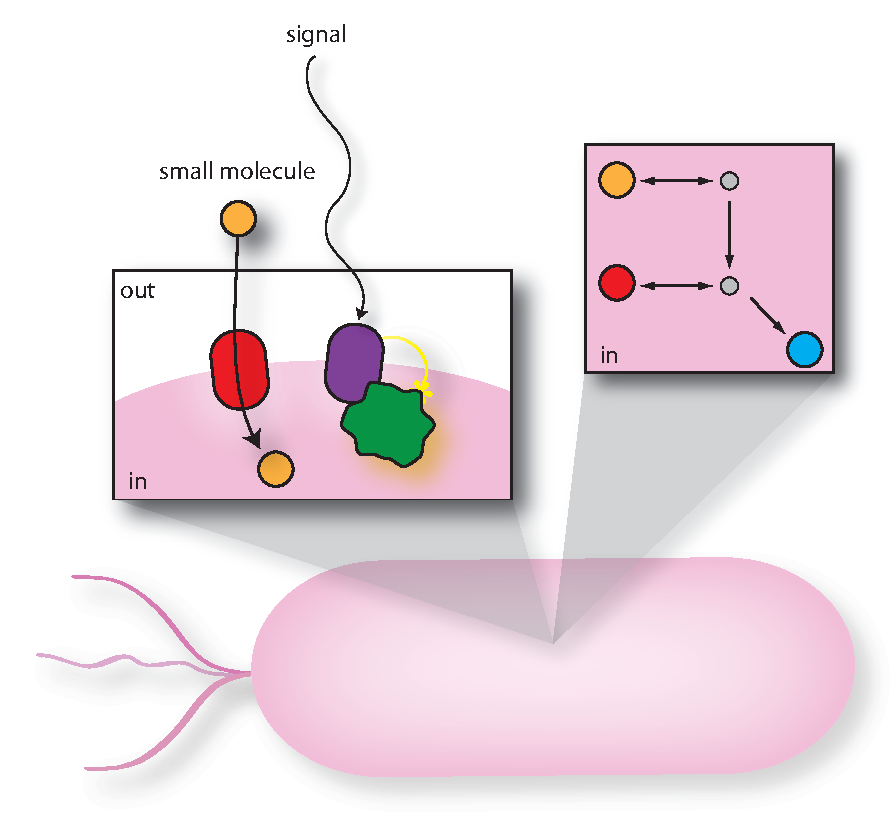
\includegraphics[width=0.6\textwidth]{figures/cell_env_signal_external}
    \caption[Microbes live in changing environments]{Microbes live in changing environments}
    \label{fig:chap1:cellsense}
\end{figure}

\begin{figure}[h!]
    \centering
    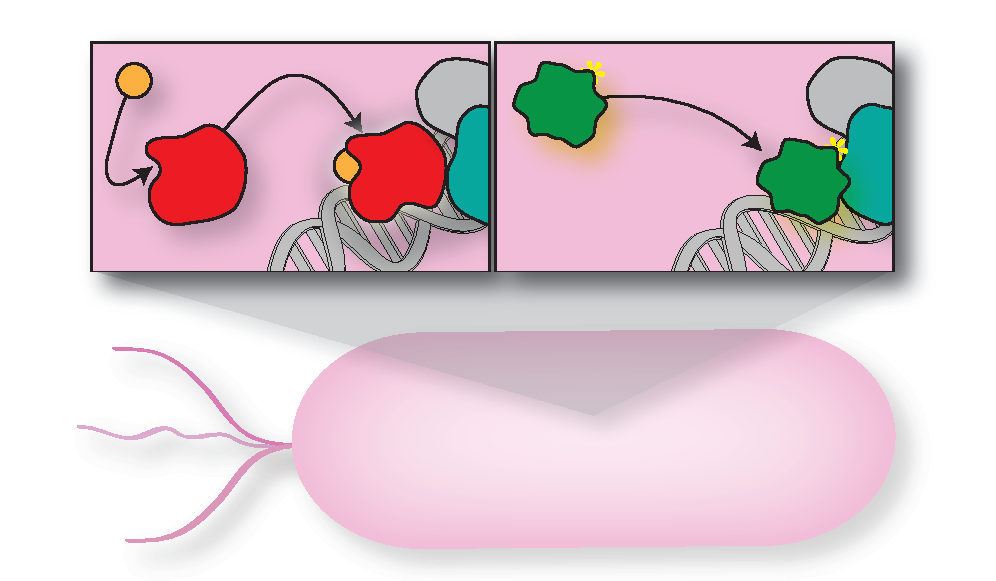
\includegraphics[width=0.6\textwidth]{figures/cell_env_internall}
 	\caption[Cells relay information to regulate the genome]{Cells relay information to regulate the genome}
    \label{fig:chap1:cellrelay}
\end{figure}

\begin{figure}[h!]
    \centering
    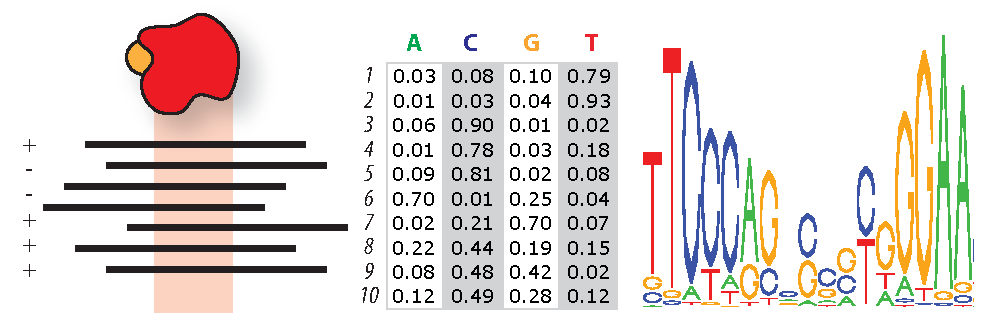
\includegraphics[width=0.9\textwidth]{figures/pssm}
 	\caption[Position specific scoring matrix (PSSM) and motif logo]{Position specific scoring matrix (PSSM) and motif logo}
    \label{fig:chap1:pssm}
\end{figure}

\begin{figure}[h!]
    \centering
    \includegraphics[width=0.6\textwidth]{figures/corem}
 	\caption[Corem: subsets of operons and regulons regulated by multiple transcription factors]{Corem: subsets of operons and regulons regulated by multiple transcription factors}
    \label{fig:chap1:corem}
\end{figure}

\begin{figure}[h!]
\centering
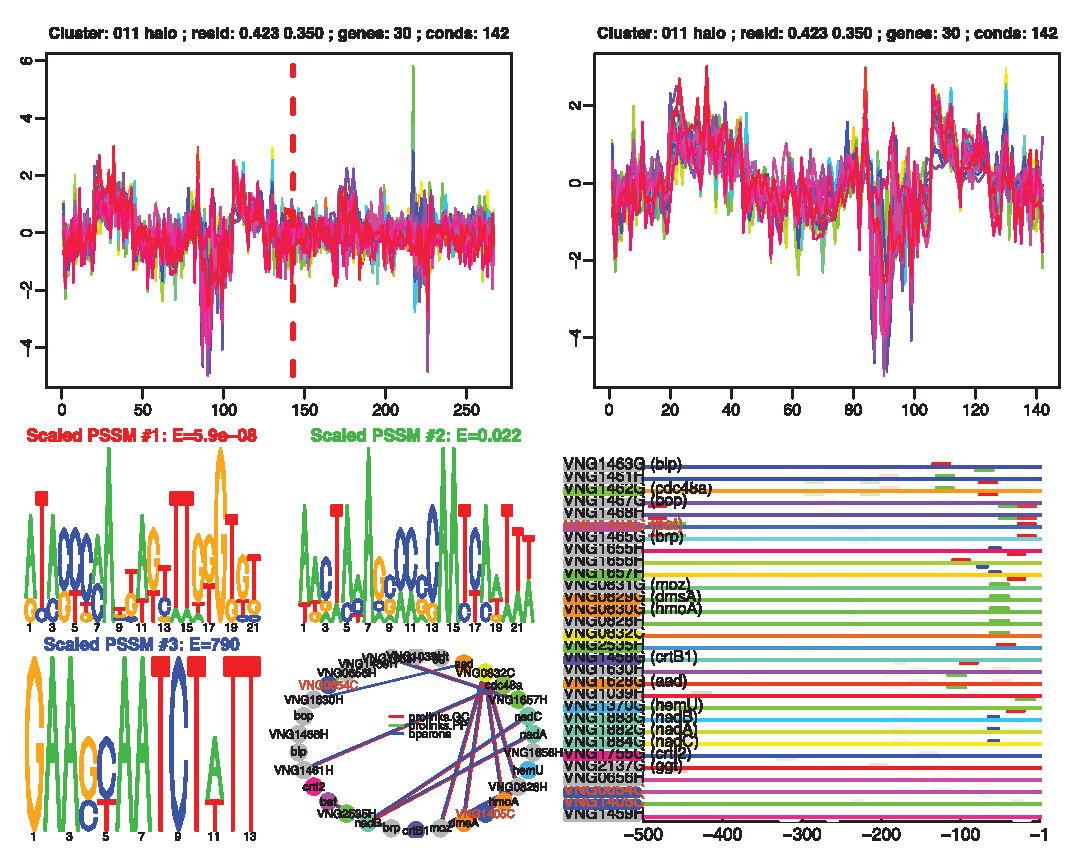
\includegraphics[width=0.9\linewidth]{figures/bicluster}
\caption[Bicluster: a conditionally co-regulated module]{Bicluster: a conditionally co-regulated module]}
\label{fig:bicluster}
\end{figure}

\begin{figure}[h!]
    \centering
    \includegraphics[width=0.9\textwidth]{figures/egrin2_fig1}
 	\caption[\egrine~Model Construction.]{\egrine~Model Construction.}
    \label{fig:egrin2:1}
\end{figure}

\begin{figure}[h!]
    \centering
    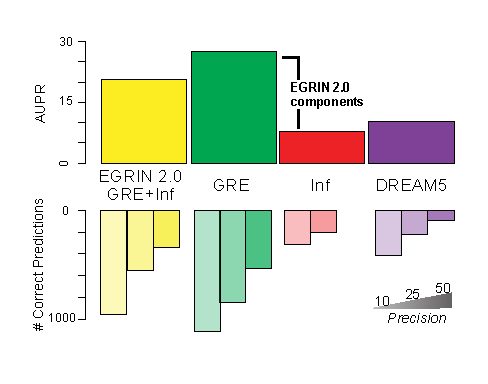
\includegraphics[width=0.75\textwidth]{figures/egrin2_AUPR}
 	\caption[\egrine~Model Validation: Performance on RegulonDB]{\egrine~Model Validation: Performance on RegulonDB}
    \label{fig:egrin2:2:A}
\end{figure}

\begin{figure}[h!]
    \centering
    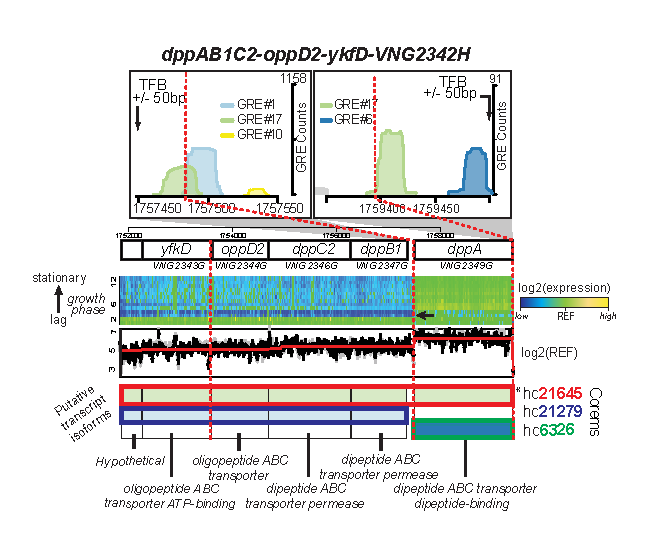
\includegraphics[width=0.8\textwidth]{figures/egrin2_dpp_1}
 	\caption[Transcriptional evidence for multiple transcript isoforms from the same operon, \halo ]{Transcriptional evidence for multiple transcript isoforms from the same operon, \halo }
    \label{fig:egrin2:3:A}
\end{figure}

\begin{figure}[h!]
    \centering
    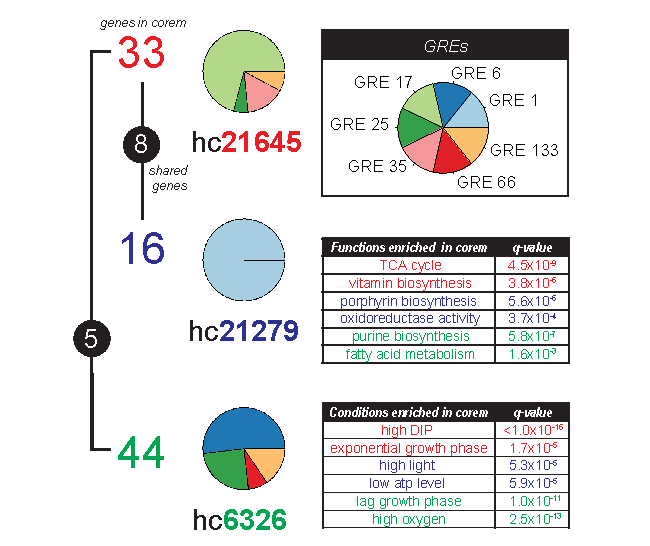
\includegraphics[width=0.65\textwidth]{figures/egrin2_dpp_2}
 	\caption[Functional consequences of multiple transcript isoforms from the same operon, \halo]{Functional consequences of multiple transcript isoforms from the same operon, \halo}
    \label{fig:egrin2:3:B}
\end{figure}


%----------------------------------------------------------------------------------------

\end{document}
